\section{Data Visualization}
\label{sec:Data Visualization}
\subsection{Dataset Description}
The Cleveland Heart Disease Dataset\cite{HeartDiseaseCleveland} originally contains 76 attributes; however, we use a preprocessed standard subset\cite{HeartDiseaseKaggle} of 13 attributes, widely utilized in published experiments with this dataset. This subset includes relevant demographic and clinical variables, described below:

The variable Age refers to the patient’s age in years, while Sex indicates the gender (1 for male, 0 for female). The type of chest pain experienced is categorized by the variable CP (Chest Pain Type), which has four categories: typical angina, atypical angina, non-anginal pain, and asymptomatic. Resting blood pressure, measured in mm Hg, is represented by Trestbps (Resting Blood Pressure), while Chol (Serum Cholesterol) records serum cholesterol levels in mg/dl.

Fasting blood sugar levels greater than 120 mg/dl are indicated by FBS (Fasting Blood Sugar), where 1 denotes true and 0 false. Resting electrocardiographic results are described by the variable Restecg (Resting Electrocardiographic Results), with values of 0 for normal, 1 for ST-T wave abnormalities, and 2 for left ventricular hypertrophy. The maximum heart rate achieved is recorded in the variable Thalach (Maximum Heart Rate Achieved), and the presence of exercise-induced angina is indicated by Exang (Exercise-Induced Angina) (1 for yes, 0 for no).

The variable Oldpeak measures ST-segment depression induced by exercise relative to rest, and Slope indicates the slope of the peak exercise ST segment. The number of major vessels (0–3) colored by fluoroscopy is indicated by the variable Ca (Number of Major Vessels Colored by Fluoroscopy), and the thalassemia test result is represented by Thal (Thalassemia Test Result), with values 3 for normal, 6 for a fixed defect, and 7 for a reversible defect. Finally, the Target variable is the outcome, indicating the presence (1) or absence (0) of heart disease.

The final column, denoted as "Target," serves as the pivotal indicator of the presence of heart disease, where a value of "0" signifies the absence of heart disease and "1" indicates its presence.

The Figure 4, illustrates the distribution of the features in the dataset, allowing us to understand their variability and potential influence on the classification task.

\begin{figure}[H]
    \centering
    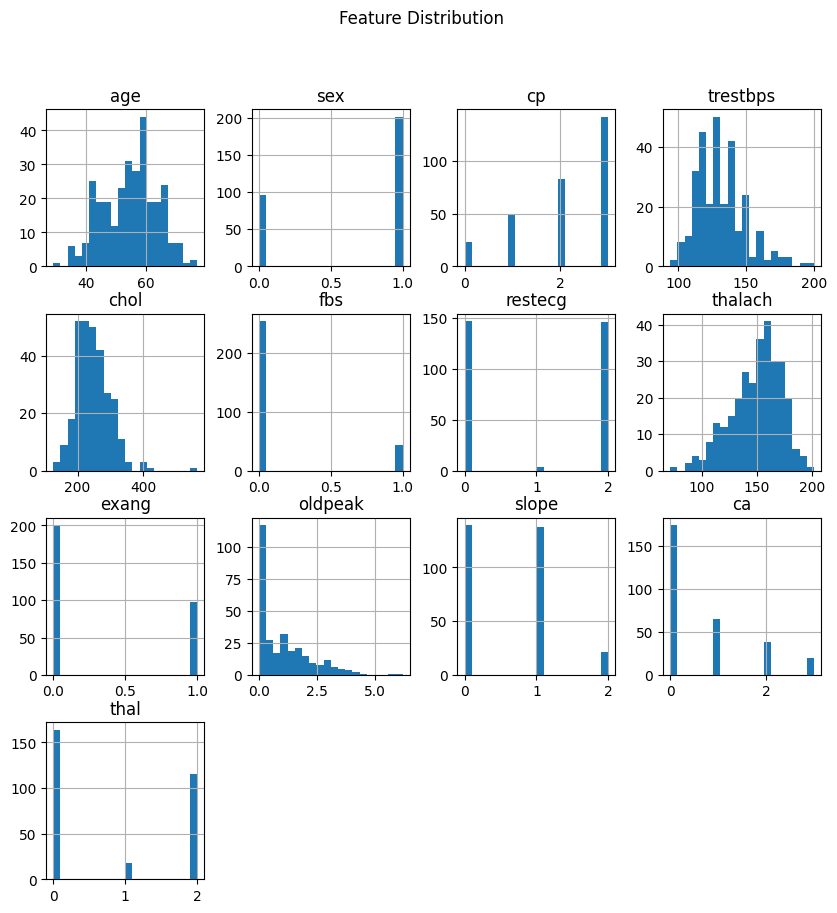
\includegraphics[width=1\linewidth]{images/feature_destribution.png}
    \caption{Feature Distribution}
    \label{fig:enter-label}
\end{figure}

\subsection{Dataset Balancing}

To gain a deeper understanding of the dataset, it is crucial to utilize various data visualization techniques, such as box plots, histograms, and scatter plots. These visualizations offer valuable insights into the relationships between variables and help identify potential patterns or correlations within the data.

The first visualization, shown in Fig. 5, is a histogram that illustrates the distribution of heart disease cases in the dataset. This histogram reveals a nearly balanced distribution, with a slight majority of patients not having heart disease. As seen in the figure, there are 160 patients without heart disease and 137 patients with heart disease, making the target variable relatively balanced. A balanced dataset is crucial for model training, as it reduces the risk of bias toward the majority class and increases the likelihood of accurate predictions.

\begin{figure}[ht] \centering 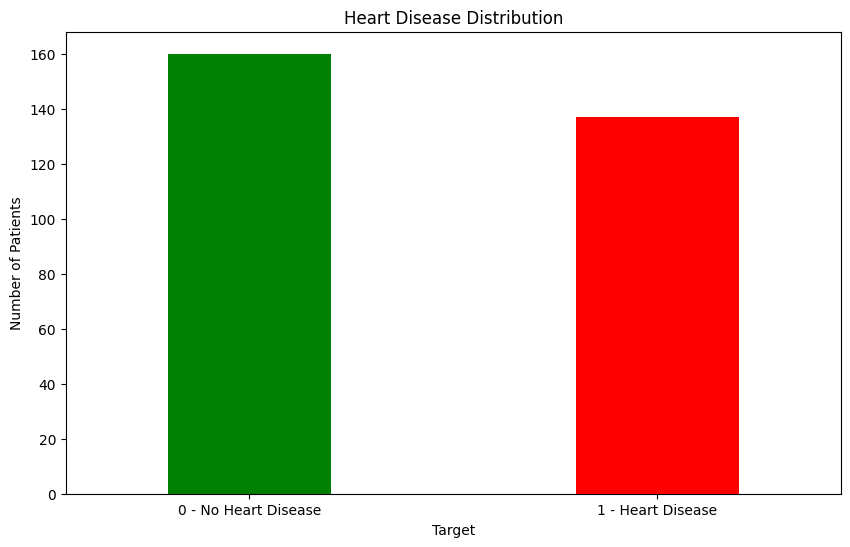
\includegraphics[width=0.8\linewidth]{images/hist_heart_desease_distribution.png} \caption{Histogram of Heart Disease Distribution} \label{fig:heart_disease_histogram} \end{figure}

The next visualization, Fig. 6, displays the distribution of patients with and without heart disease in a circular format (pie chart). This provides a clearer view of the proportions of each class. The dataset is balanced, with 53.87\% of patients without heart disease and 46.13\% of patients with heart disease.

\begin{figure}[ht] \centering 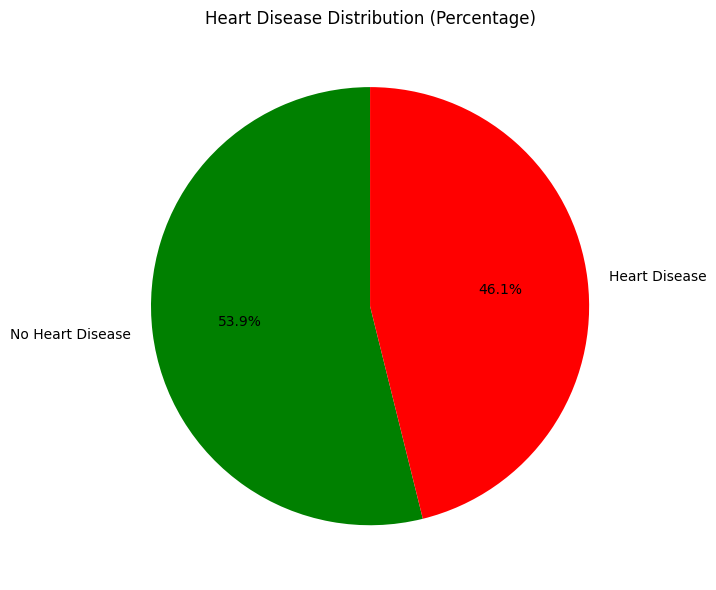
\includegraphics[width=0.75\linewidth]{images/heart_distribution_circular.png} \caption{Heart Disease Distribution (Percentage)} \label{fig:heart_disease_pie_chart} \end{figure}

This balance is important to ensure that the model does not develop a bias towards predicting the majority class, allowing for more accurate and fair predictions.

\subsection{Comparison of Age and Sex Distribution in the Dataset}
The age distribution, Fig. 7, shows that the average age of the patients is 54.54 years, with the median being 56 years, and the most frequent age (mode) being 58 years. The age range spans from 29 years to 77 years, indicating a relatively broad age distribution within the dataset. This diversity in age is important for creating a model that can effectively predict heart disease across different age groups.

\begin{figure}[ht]
    \centering
    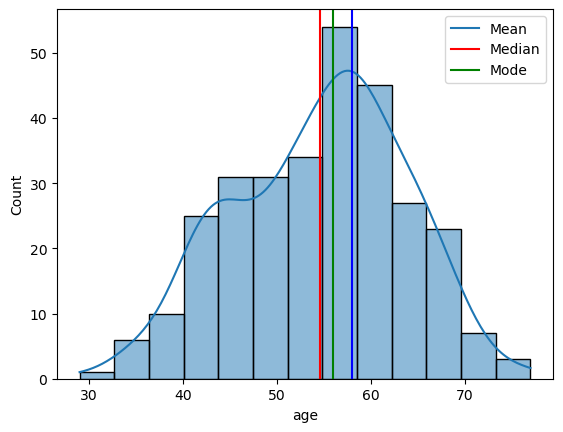
\includegraphics[width=0.8\linewidth]{images/age_distribution.png}
    \caption{Age Distribution}
    \label{fig:enter-label}
\end{figure}
\hfill \break

Notably, a significant number of patients fall within the 40 to 70-year-old range, which is typically the period when heart diseases are more commonly diagnosed. This trend is consistent with general medical knowledge, as the risk of heart disease increases with age, particularly after the age of 40. Contributing factors include the accumulation of cardiovascular risk factors over the years, such as high blood pressure, cholesterol levels, and lifestyle choices. This concentration of patients in the 40–70 age range suggests that the dataset captures a critical age group for heart disease prediction.

\begin{figure}[ht]
    \centering
    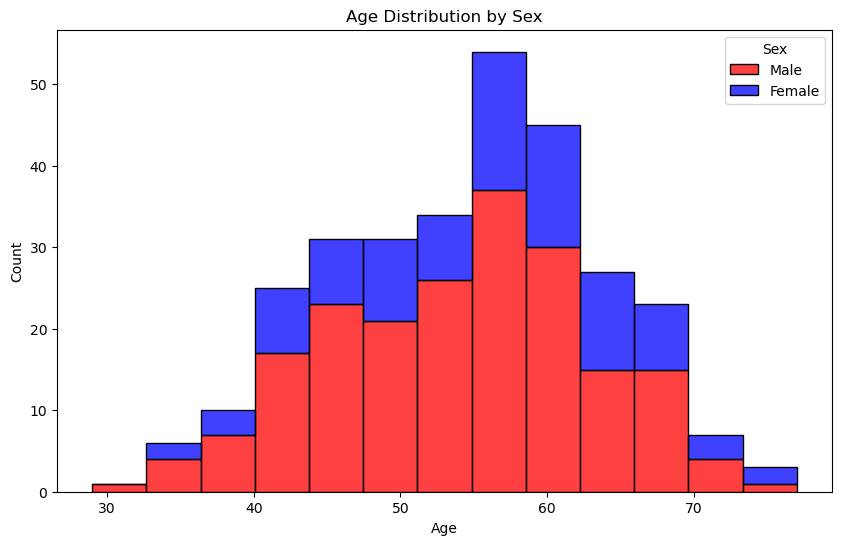
\includegraphics[width=0.8\linewidth]{images/women_men.png}
    \caption{Age distribution by Sex}
    \label{fig:enter-label}
\end{figure}

When we look at the age distribution by sex on figure 8, we observe that the dataset contains 201 men (67.7\% of the total) and 96 women (32.3\% of the total). This reveals a higher representation of men in the dataset. Men, on average, are more likely to develop heart disease than women, which is reflected in the dataset's demographic distribution.

\begin{figure}[ht]
    \centering
    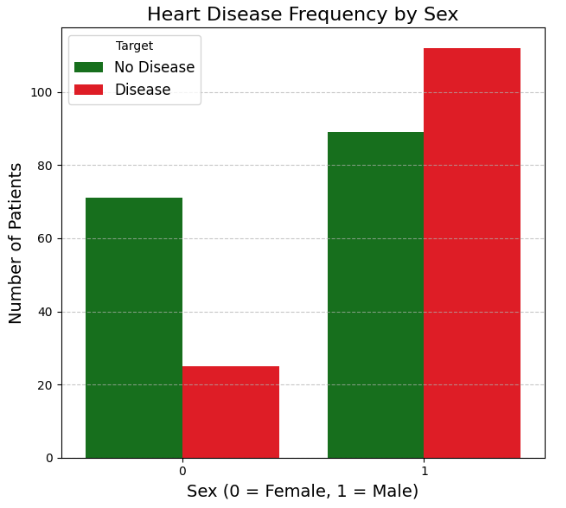
\includegraphics[width=0.75\linewidth]{images/freq_heart_disease_by_sex.png}
    \caption{Heart Disease Distribution by Sex }
    \label{fig:enter-label}
\end{figure}

Among the men, 55.7\% have heart disease, while 44.3\% do not. In contrast, among the women, only 26.0\% have heart disease, with the remaining 74.0\% without it. These figures highlight that heart disease is more prevalent among men in this dataset, which is consistent with general clinical findings that heart disease tends to affect men at a higher rate.
%\hfill \break
\begin{figure}[H]
    \centering
    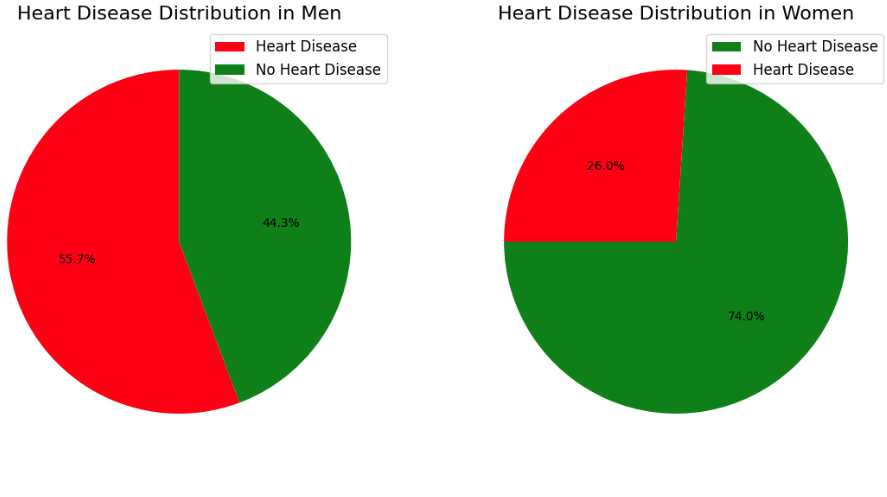
\includegraphics[width=1\linewidth]{images/perc_disease_by_sex.png}
    \caption{Heart Disease Distribution by Sex (Percentage)}
    \label{fig:enter-label}
\end{figure}

Further examining the age distribution within each sex, we can observe how age interacts with heart disease for both men and women. Heart disease is present in a notable portion of the male and female population particularly in the older age groups. While heart disease is less common in women overall, it is still present in a notable portion of the female population.

In summary, the data shows that men are more likely to have heart disease than women, and age plays an important role in the development of the disease for both genders. This insight helps us understand the potential impact of age and sex on heart disease prediction models and may guide future analyses on how to best predict heart disease based on these factors.

\subsection{Attribute Distributions and Their Relationship with Heart Disease} 

The dataset reveals notable differences in the distributions of key attributes between patients with and without heart disease, as seen in figure 11 and 12. These distinctions highlight critical factors that may be associated with the presence of heart disease, providing valuable insights for diagnosis, risk assessment, and preventive strategies.

\begin{figure}[!htb]
    \centering
    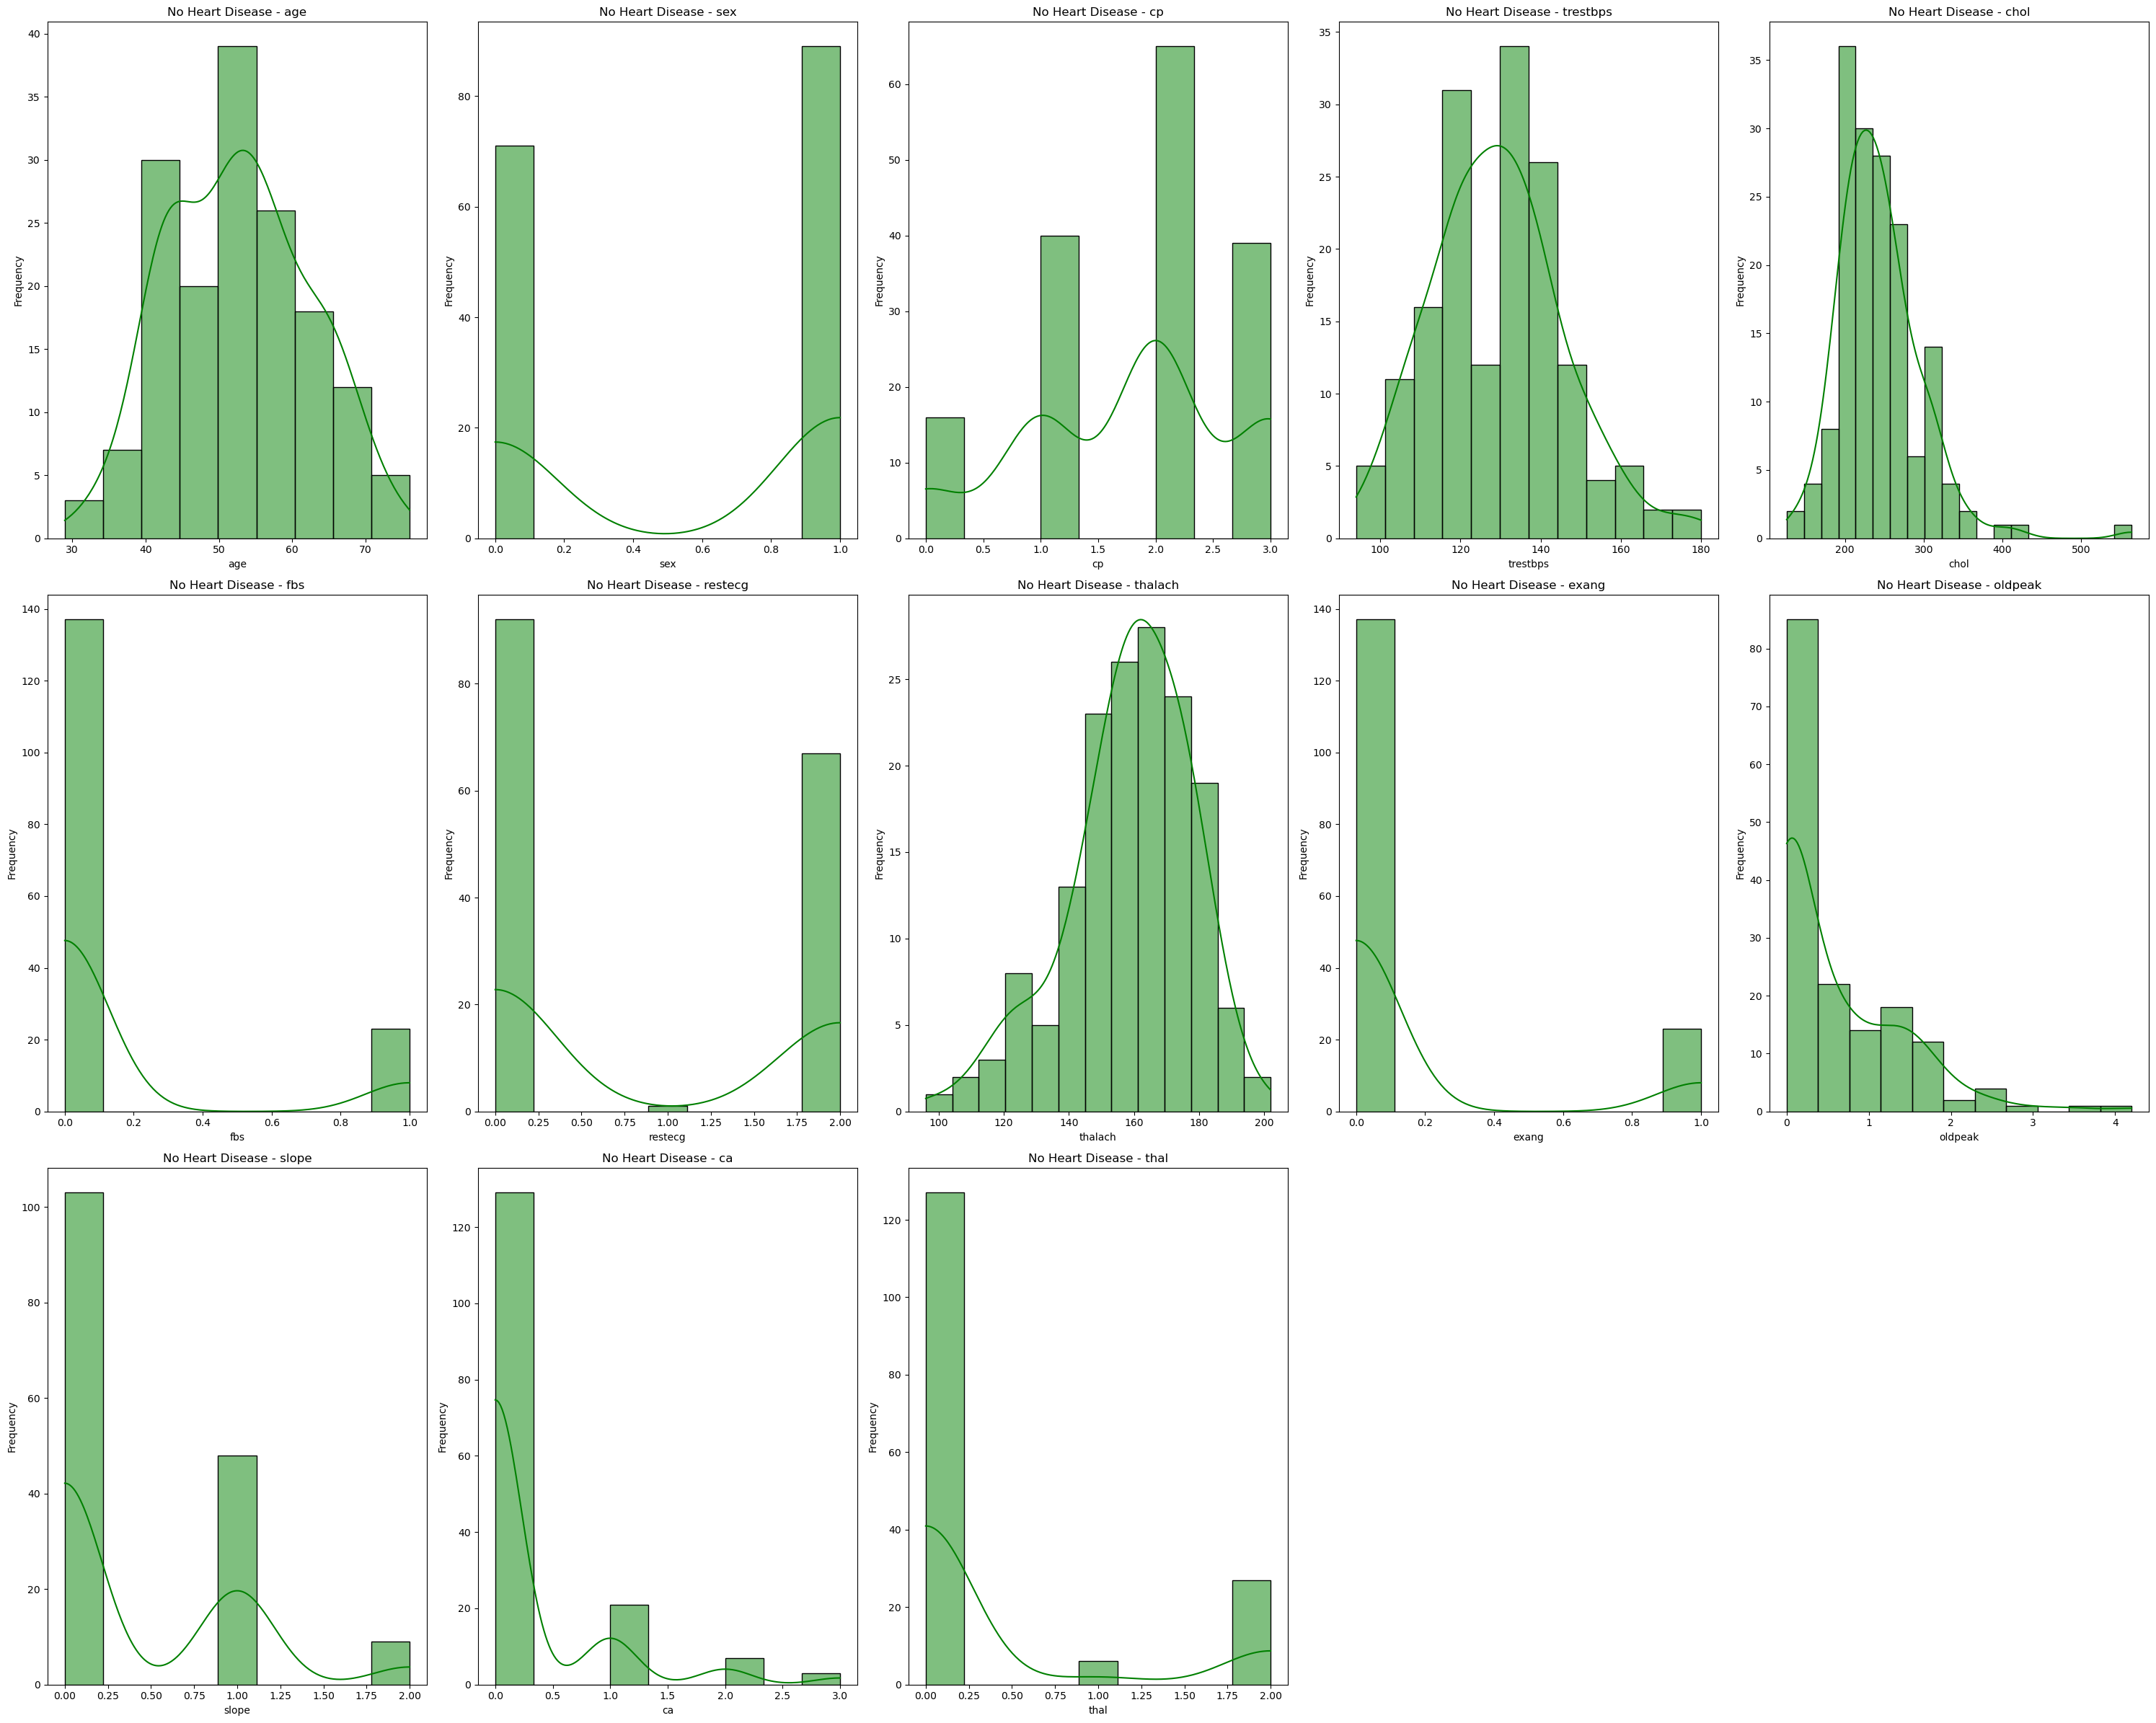
\includegraphics[width=1\linewidth]{images/no_heart_distribution.png}
    \caption{Distribution of patients healthy patients (without heart disease)}
    \label{fig:no_heart_distribution}
\end{figure}

\begin{figure}[!htb]
    \centering
    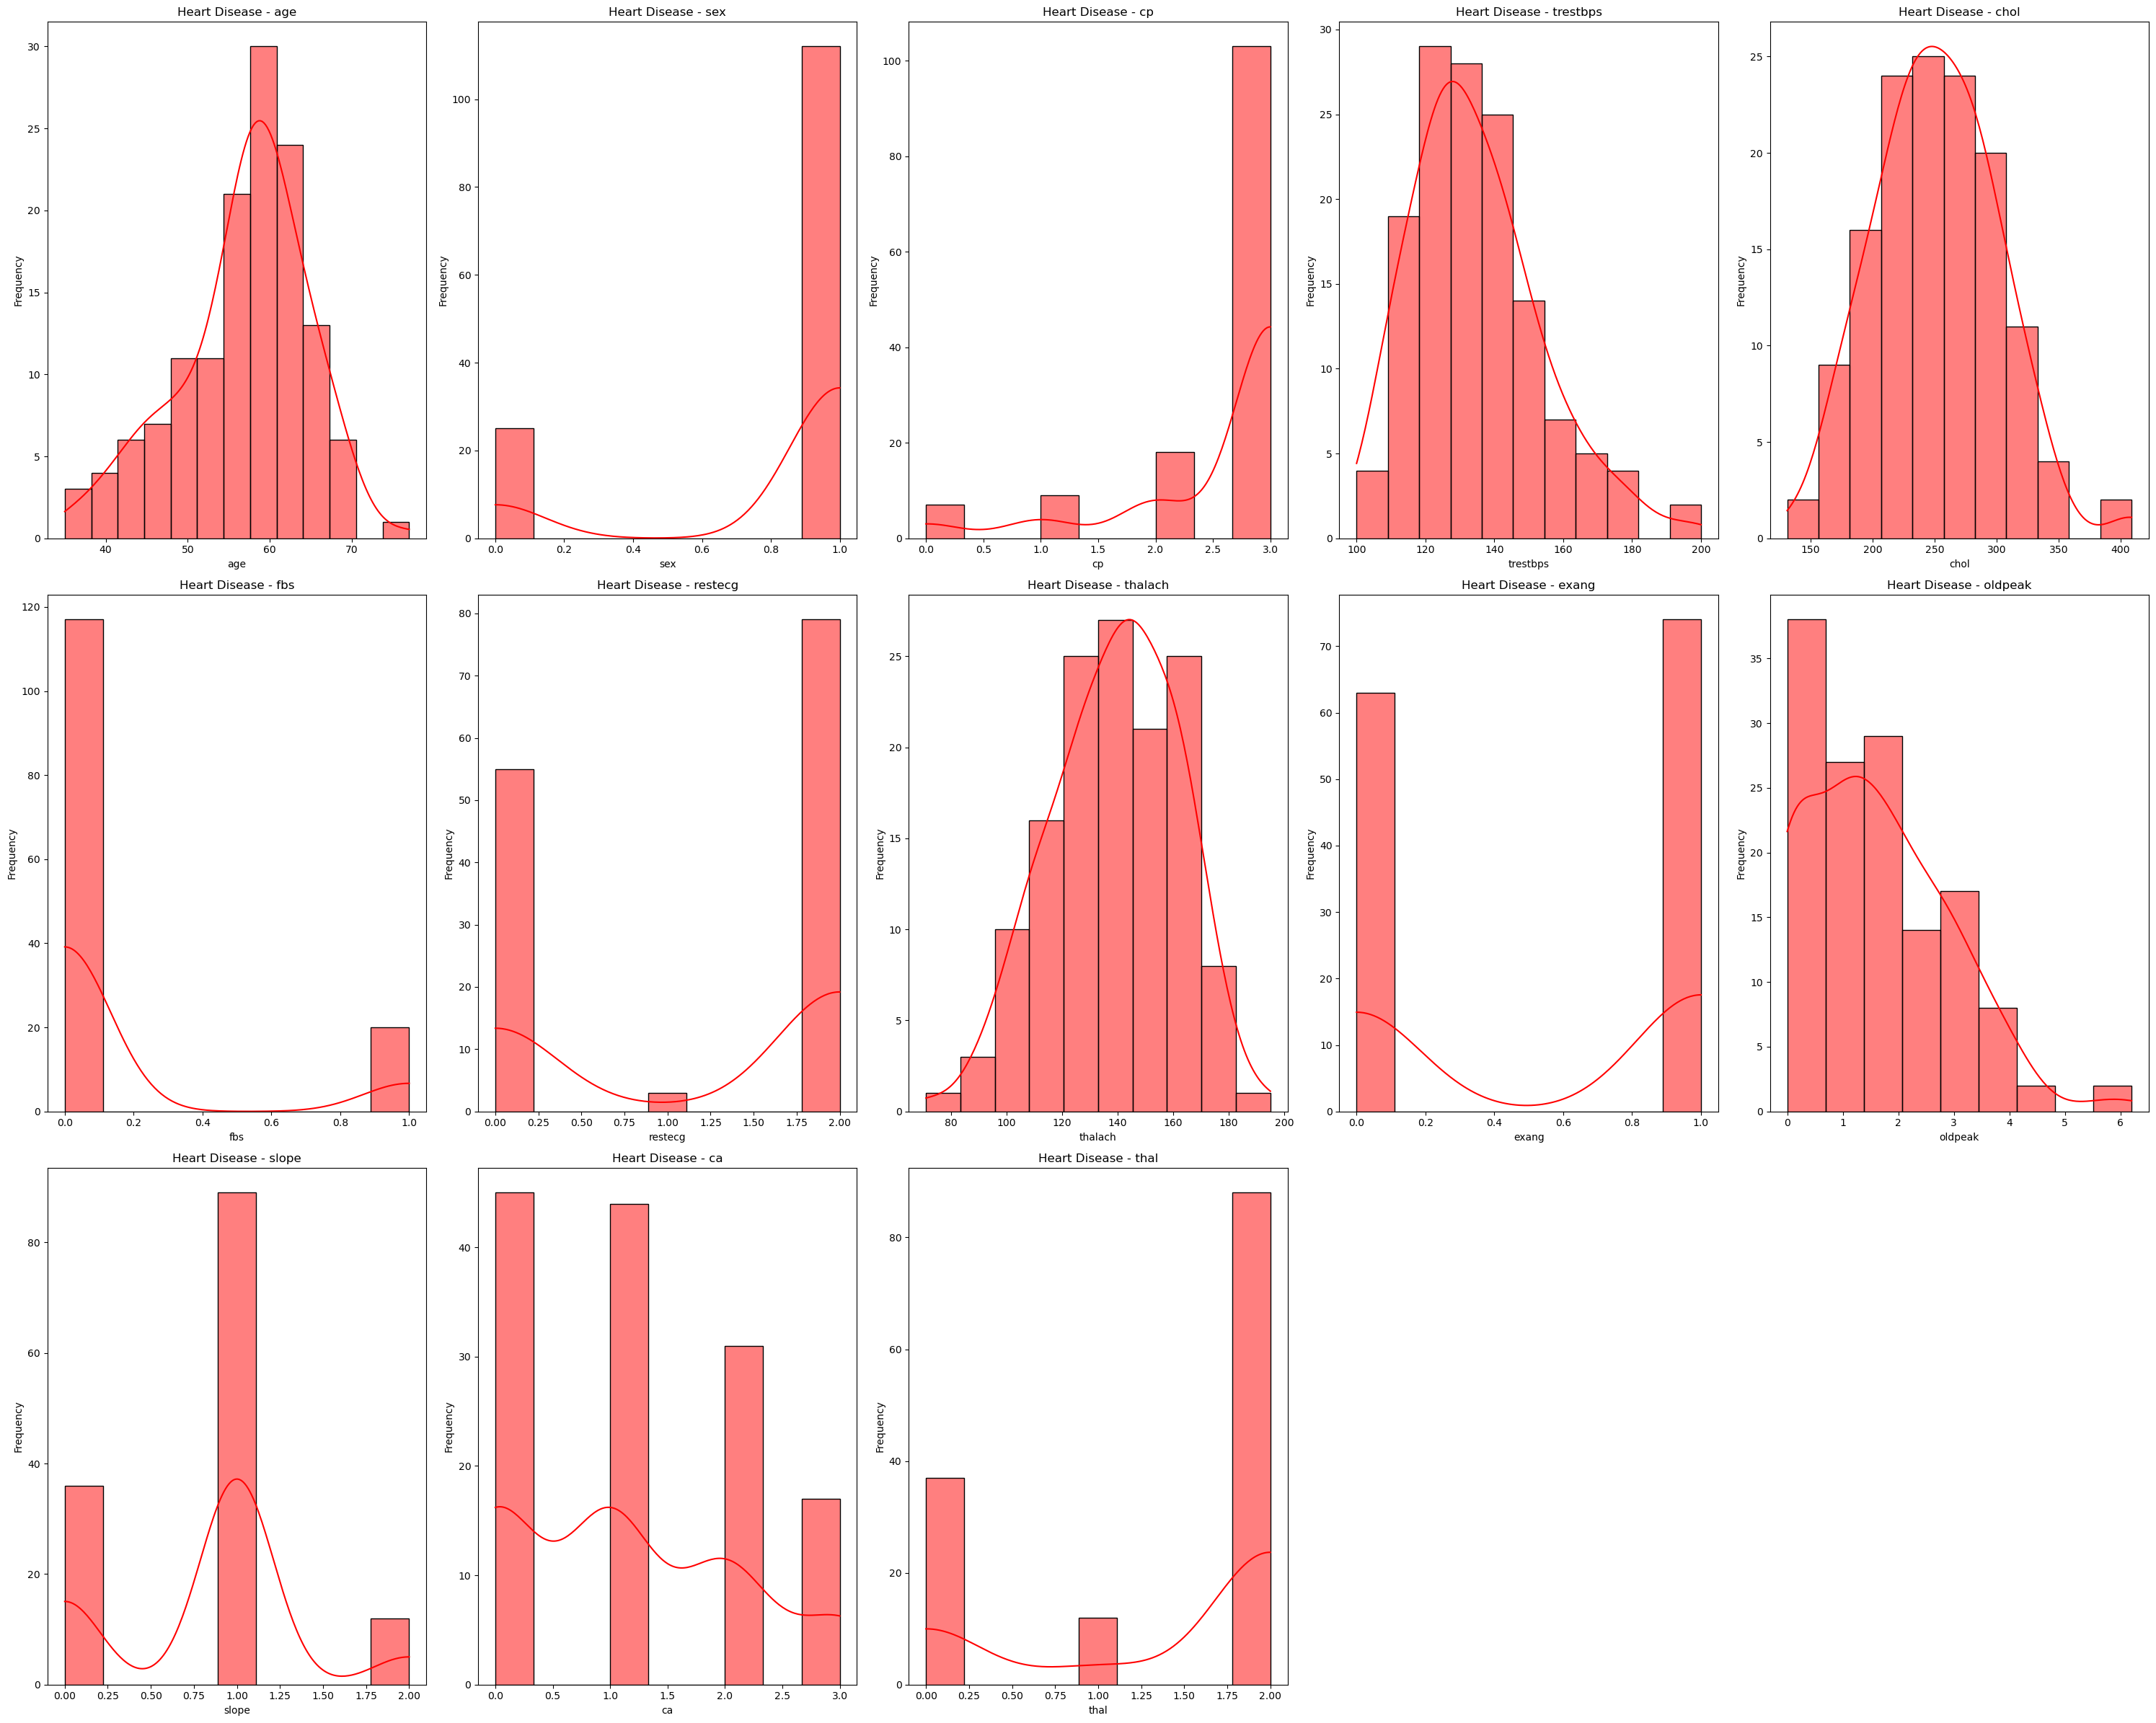
\includegraphics[width=1\linewidth]{images/heart_distribution.png}
    \caption{Distribution of patients with heart disease}
    \label{fig:heart_distribution}
\end{figure}

\begin{enumerate}
    \item Age Distribution:
 Patients with heart disease show a clear peak in the 60–70-year age range, reflecting a higher prevalence of the condition in older individuals. In contrast, patients without heart disease display a more uniform age distribution, indicating less dependency on age in this group.

    \item Sex Distribution:
 The group with heart disease has a significantly higher proportion of male patients compared to the group without heart disease. This aligns with the well-documented higher risk of heart disease in men.

    \item Chest Pain Type (CP) Distribution:
Among patients with heart disease, the distribution of chest pain types has a high peak at the highest value of CP. This suggests that this specific type of chest pain is strongly associated with the presence of heart disease. In comparison, the no heart disease group shows a more uniform distribution across CP types.

    \item Resting Blood Pressure (Trestbps) Distribution:
The heart disease group exhibits a slightly more right-skewed distribution of resting blood pressure values.

    \item Serum Cholesterol (Chol) Distribution:
Even though the cholesterol levels among patients with heart disease tend to be right-skewed, with higher values compared to those without heart disease, in our dataset both the groups of diseased and healthy patients have an even distribution of this measure.

    \item Slope of the Peak Exercise ST Segment Distribution:
 The slope distribution in the heart disease group is unimodal with a peak at the flat category of slope. A flat or horizontal ST segment depression during exercise stress testing is often considered abnormal. It suggests myocardial ischemia, which occurs when there is insufficient blood flow to the heart muscle during stress, typically due to atherosclerotic coronary artery disease. In contrast, the no heart disease group have the most frequency in the upsloping category suggesting that they are healthy individuals. 
\end{enumerate}

These differences in attribute distributions between the two groups highlight the importance of factors such as age, sex, chest pain type, blood pressure, cholesterol levels, and exercise-induced ST segment slope in identifying and assessing the risk of heart disease. Understanding these patterns not only aids in distinguishing between individuals with and without the condition but also provides a foundation for more targeted diagnostic and preventive approaches.

\subsection{Correlation Matrix Insights} 
The correlation matrix present in Fig. 13 reveals important relationships between the attributes and the target variable. 
\begin{figure}[H]
    \centering
    \includegraphics[width=1\linewidth]{images/matriz_correçacao.png}
    \caption{Correlation Matrix}
    \label{fig:enter-label}
\end{figure}

These can help in the process of feature selection and model development for heart disease prediction:
\begin{itemize}
    \item Age has a moderate positive correlation (0.23) with the target, indicating that the likelihood of heart disease increases with age.
    \item Sex also shows a moderate positive correlation (0.28) with the target, suggesting that being male is associated with a higher risk of heart disease.
    \item Chest Pain Type (CP) has a moderately strong positive correlation (0.41), implying that specific chest pain types are more indicative of heart disease.
    \item Thalach (Maximum Heart Rate Achieved) shows a moderately strong negative correlation (-0.42), indicating that lower maximum heart rates are associated with a higher risk of heart disease.
    \item Exercise-Induced Angina (Exang) and Oldpeak (ST Depression) both have a moderately strong positive correlation (0.42) with the target, highlighting their significance in heart disease prediction.
    \item Ca (Number of Major Vessels Colored by Fluoroscopy) has a positive correlation (0.46), making it one of the stronger predictors of heart disease.
    \item Thal (Thalassemia) demonstrates the strongest positive correlation (0.52) with the target, indicating its significant role in predicting heart disease.
\end{itemize}

Additional Observations:

\begin{itemize}
    \item Attributes such as Chol (Serum Cholesterol) and Trestbps (Resting Blood Pressure) have low positive correlations (0.08 and 0.15, respectively), suggesting limited predictive power when considered individually.
    \item Fbs (Fasting Blood Sugar) shows a near-zero correlation (0.00), implying minimal influence on heart disease prediction in this dataset.
    \item Several attributes, including Slope, Restecg, and Oldpeak, exhibit moderate correlations with one another (e.g., Slope and Oldpeak: 0.58), indicating potential interactions that could enhance predictive modeling.
\end{itemize}

While some attributes show strong linear relationships with the target, many exhibit low correlations (< 0.3). This suggests that more complex modeling techniques may be required to capture non-linear relationships and interactions among the attributes for accurate heart disease prediction.